
\documentclass[12pt, oneside]{amsart}
\usepackage[font={sf}]{caption}
\usepackage[]{graphics}
\usepackage{graphicx}
\usepackage{epstopdf}
\usepackage{hyperref}
\hypersetup{breaklinks=true, colorlinks=true, citecolor=blue}
\usepackage{natbib}
\usepackage{color}
\usepackage{soul}
\usepackage{rotating}
\usepackage{tabularx}
\usepackage{longtable}
\usepackage{lscape}
\usepackage{array}
\usepackage{multirow}
\usepackage{setspace}
\usepackage{textcomp}
\usepackage{dcolumn}
\setlength{\LTcapwidth}{6in}
\usepackage{dcolumn}
\usepackage[margin=1in]{geometry}

 \bibpunct{(}{)}{,}{a}{}{,}
 \doublespacing
 \raggedright
 \setlength{\parindent}{15pt} 


\begin{document}
%\setcounter{secnumdepth}{0}


{ \Large \bf Supplementary Figures}

Lotterhos et al. 2017. (Add Title Here). Methods in Ecology and Evolution.

\hspace{3cm}

%\tableofcontents
%\listoftables
%\renewcommand\thesection{S1}
%\listoffigures

\renewcommand{\figurename}{Supplementary Figure}

\begin{figure}[h]
\begin{center}
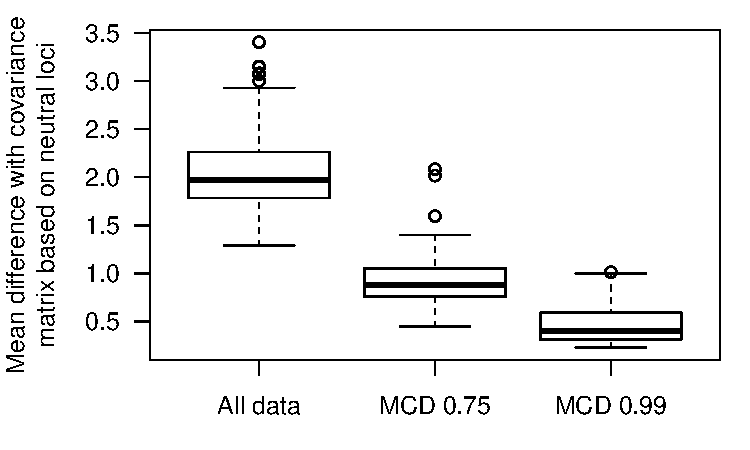
\includegraphics[width=4in]{../figures_man2/S1-LandsharcCompareToNeutralCovMat.pdf}
\end{center}
\caption[]{Comparison of the mean absolute difference between the variance-covariance matrix among the univariate statistics calculated using (i) all the data, (ii) the MCD estimate using 75\% of the dataset, and (iii) the MCD estimate using 99\% of the dataset.  Boxplots are summarized over all demographies and sampling designs.

{\bf TO DO: Should I switch MCD99 and MCD75 here, since MCD99 will be closer to "all data" than MCD75?}
} 
 \label{fig:???}
\end{figure}



\newpage
\begin{figure}[h]
\begin{center}
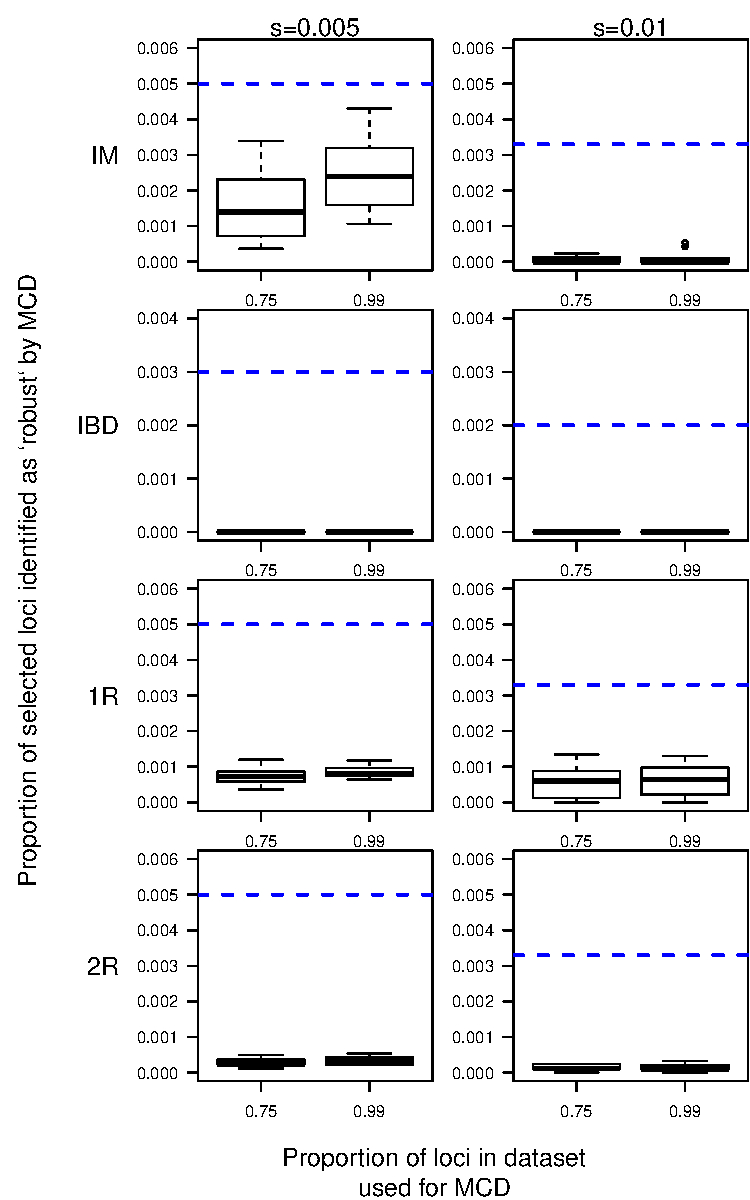
\includegraphics[height=6in]{../figures_man2/S2-LandsharcProportionSelectedMCD.pdf}
\end{center}
\caption[]{Evaluation of whether loci affected by selection were identified as 'robust' points (e.g., not outliers) by the MCD algorithm. Loci under relatively weak selection (s=0.005) are in the left column, well loci under moderate selection are in the right column (s=0.01). The horizontal dashed line represents the null expectation, based on the proportion of loci under that strength of selection in the entire dataset. The MCD never identified loci simulated under strong selection (s=0.1) as robust (expected = 0.001 in IBD and 0.0017 in IM, 1R, and 2R; observed = 0 across all simulations).} 
 \label{fig:???}
\end{figure}




\newpage
\begin{figure}[h]
\begin{center}
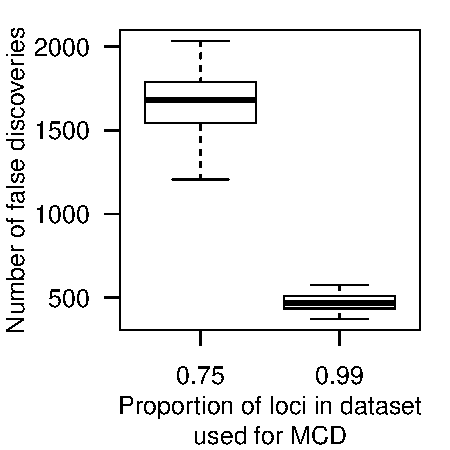
\includegraphics[width=4in]{../figures_man2/S3-LandsharcFalsePositivesMCD.pdf}
\end{center}
\caption[]{The number of false discoveries (neutral loci inferred to be outliers, out of 9900 total neutral loci in the dataset) resulting if robust points identified by the MCD are used as an empirical null distribution.} 
 \label{fig:???}
\end{figure}

\newpage
\begin{figure}[h]
\begin{center}
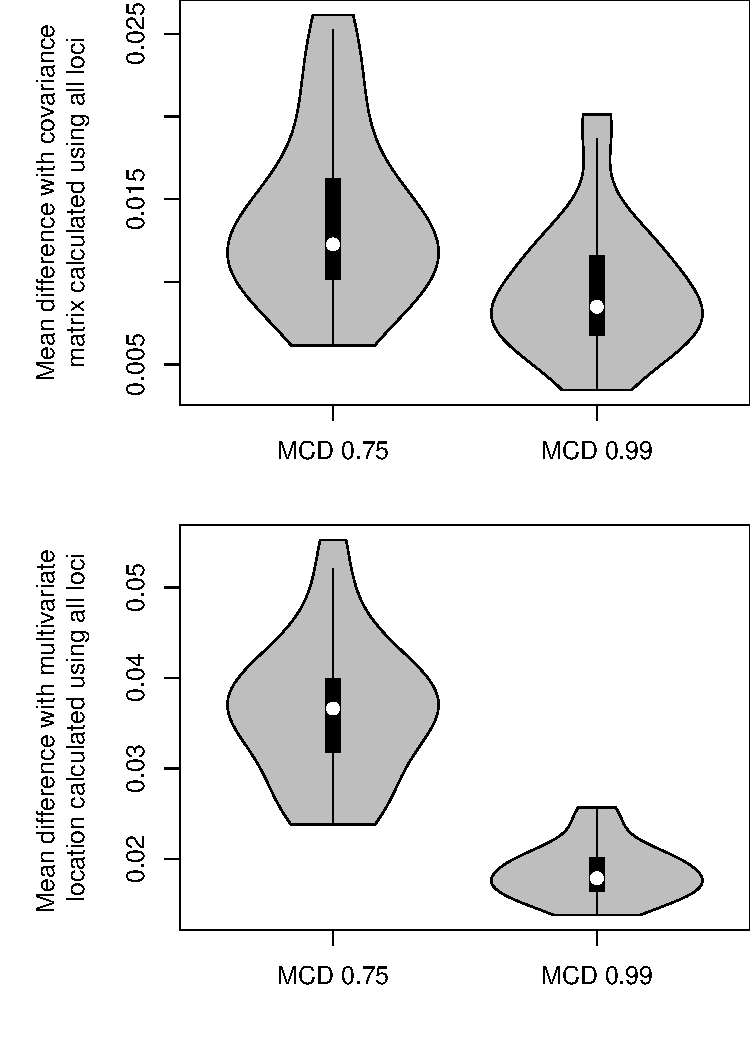
\includegraphics[width=4in]{../figures_man2/S4-DogDataCompareLocationScatter.pdf}
\end{center}
\caption[]{A comparison of the mean difference in the multivariate location (mean) and scatter (covariance) on the dog dataset based on the robust points identified by the MCD algorithm compared to that based on all the data.} 
 \label{fig:???}
\end{figure}

\newpage
\begin{figure}[h]
\begin{center}
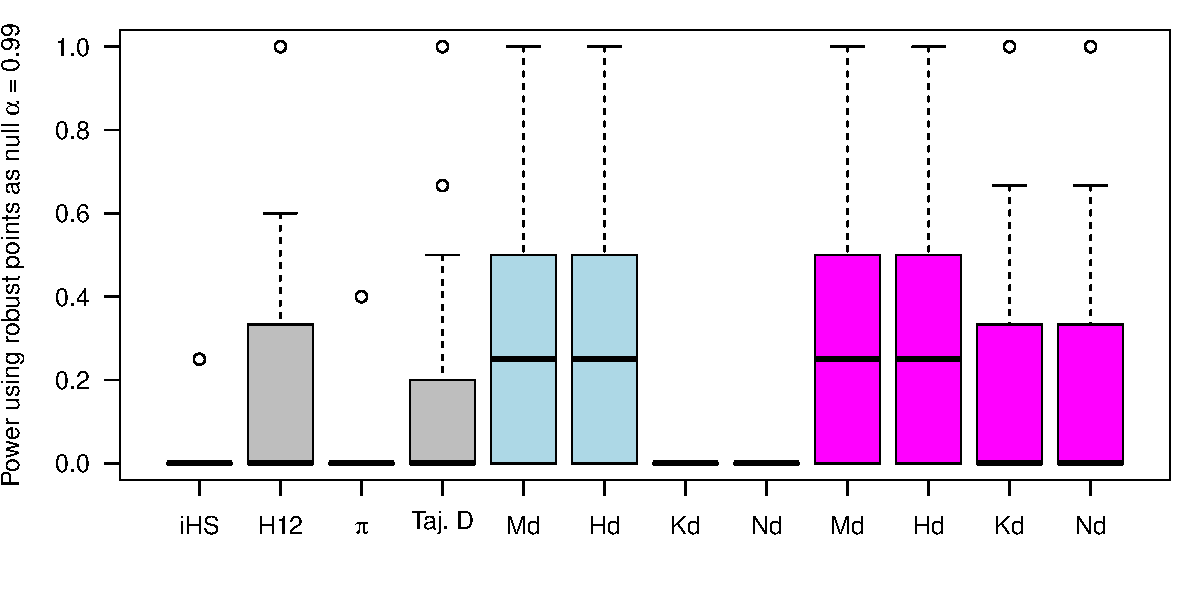
\includegraphics[width=4in]{../figures_man2/S5-DogPower_alpha099.pdf}
\end{center}
\caption[]{Comparison of power of different univariate and multivariate statistics to detect known QTL in the dog dataset. Power was evaluated as the proportion of known QTL with a signal above the maximum value of that statistic at the robust points identified by the MCD with $\alpha=0.75$. Multivariate "default" was calculated using all the data (same as Figure 4 in the main paper), while "MCD" was calculated using the MCD estimates of multivariate mean and covariance as well as the robust points in the calculation, if applicable. Statistics evaluated include integrated haplotype score (iHS), H12, Tajima's D (Taj. D), nucleotide diversity ($\pi$), Mahalanobis distance (Md), harmonic mean distance (Hd), kernel deviance (Kd), and nearest neighbor distance (Nd).} 
 \label{fig:???}
\end{figure}


\end{document}